\section*{Math 202A - HW12 - Dan Davison - \texttt{ddavison@berkeley.edu}}

Recall that for locally integrable $f$, the average value of $f$ on a ball centered at $x$ is
\begin{align*}
  (A_r f)(x) = \frac{1}{m(B(x, r))} \int_{B(x, r)} f,
\end{align*}
and that the maximal function $(H f)(x) := \origsup_r (A_r |f|)(x)$ is the maximum average value of $|f|$ over
balls of any size centered at $x$.

The main theorem concerning $H f$ is

\begin{theorem}[Maximal theorem]
  For any $f \in L^1$ there exists a constant $C > 0$ such that for all $a > 0$
  \begin{align*}
    m\(\{x ~:~ (H f)(x) > a\}\) \leq \frac{C}{a} \int |f|.
  \end{align*}
\end{theorem}
\begin{mdframed}
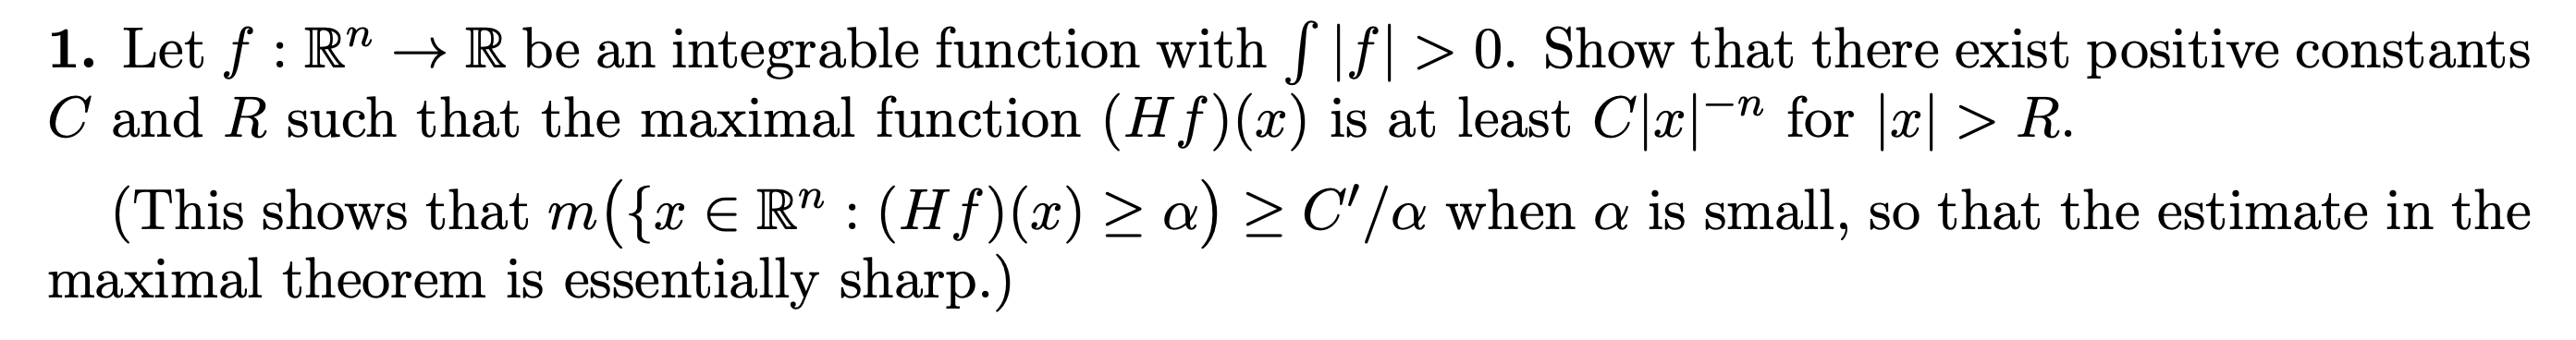
\includegraphics[width=400pt]{img/analysis--berkeley-202a-hw12-1ffa.png}
\end{mdframed}

Informally, the claim is that beyond some distance $R$ from the origin, the maximum average value of $|f|$ seen
from a point further from the origin is capable of being lower than that seen from a point closer to the
origin. Why would this be? Suppose we have points $x_1$ and $x_2$ with $|x_2| > |x_1|$, and that we are located
at $x_2$.

I think the intuition is this: since $0 < \int |f| < \infty$, there must exist some distance $U$ such
that $|f(x)|$ is small/decaying rapidly to zero for all $|x| > U$. Viewed from out there, $(H f)(x)$ is
determined by what proportion the bulk of the mass (closer to the origin) makes up, and this decreases
as $|x|^{-n}$.




\begin{proof}
  We must show that $(H f)(x) \geq C|x|^{-n}$ for $|x| > R$, where $C$ and $R$ are constants to be determined.

  Let $M = \int |f| \in (0, \infty)$.

  Let $\eps > 0$.

  First suppose $f = M\ind_{[-\eps, \eps]}$.

  Then we have $(H f)(x) \to C|x|^{-n}$ as $|x|\eps^{-1} \to \infty$, where $C$ is a constant that reflects
  both $M$ (the mass near the origin) and the volume of a ball of radius $|x|$.

  \red{TODO} give an explicit expression for the volume

\end{proof}

\newpage
\begin{mdframed}
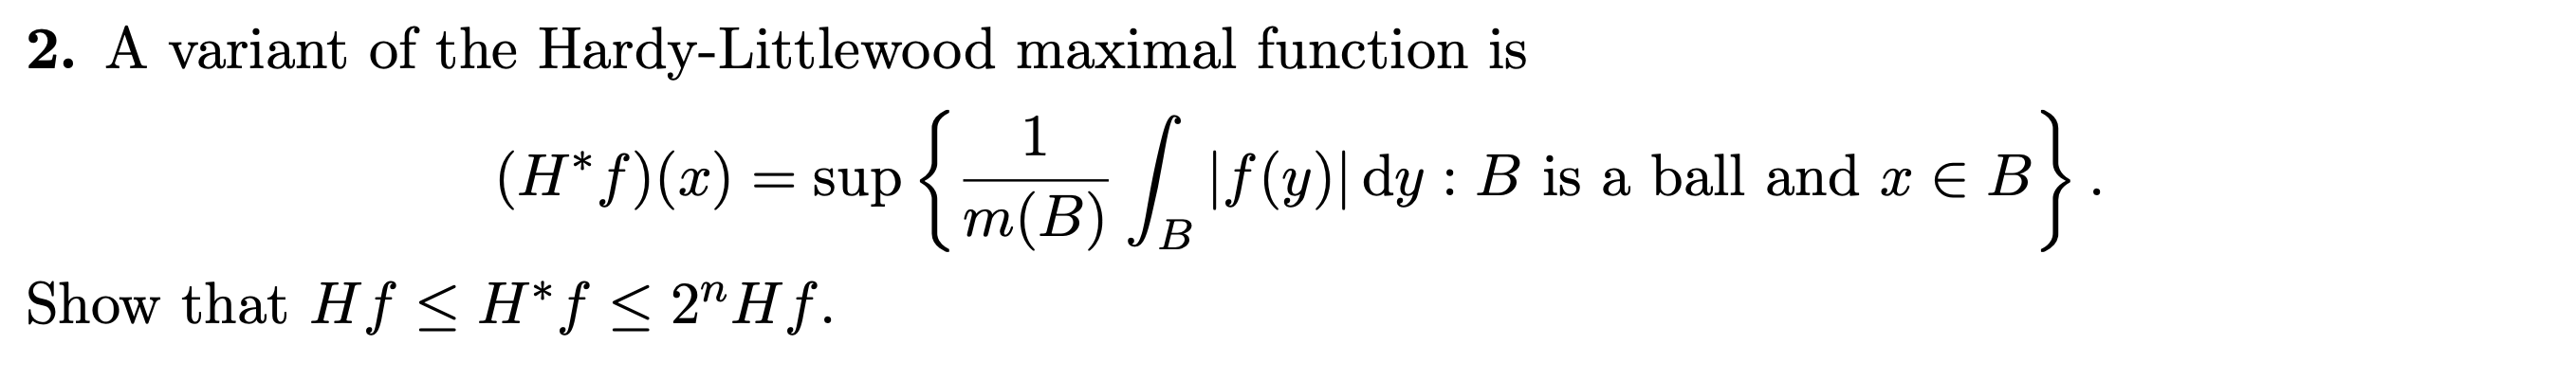
\includegraphics[width=400pt]{img/analysis--berkeley-202a-hw12-5314.png}
\end{mdframed}

\begin{proof}
  Define
  \begin{align*}
    U(x) &:= \Big\{(A_r |f|)(x) ~:~ r > 0\Big\} \\
    V(x) &:= \Big\{(A_r |f|)(x') ~:~ r > 0, x' \in (x - r, x + r)\Big\}.
  \end{align*}
  By definition
  \begin{align*}
    (H f)(x) := \sup U(x),
  \end{align*}
  and
  \begin{align*}
    (H* f)(x) := \origsup V(x).
  \end{align*}
  Note that $U(x) \subseteq V(x)$ for all $x$. Therefore $H f \leq H^* f$.

  It remains to show that $H^* f \leq 2^n H f$.

  Let $x$ be a point in the domain of $f$.

  Let $\eps > 0$ and let $x', r$ be such that $(H^* f)(x) - (A_r |f|)(x') < \eps$. (Informally, $B(x', r)$ is a
  maximizing ball in the computation of $(H^* f)(x)$, up to a small error of $\eps$.)

  Suppose $|x - x'| = r$ and consider the ball $B(x, 2r) \supseteq B(x', r)$. The most extreme difference
  possible between $(A_{2r} |f|)(x)$ and $(A_r |f|)(x')$ occurs when $f = 0$ on $B(x, 2r)$. In that case we
  have $(A_{2r} |f|)(x) = \frac{1}{2^n}(A_r |f|)(x)$ (informally, the two balls overlap in one hemisphere, and
  on the other hemisphere there is no overlap and we penalize as much as we can).

  \red{TODO} the balls don't overlap exactly for $n > 1$, be explicit or estimate this.

  Therefore $H^* f \leq 2^n H f$.
\end{proof}

\newpage
\begin{mdframed}
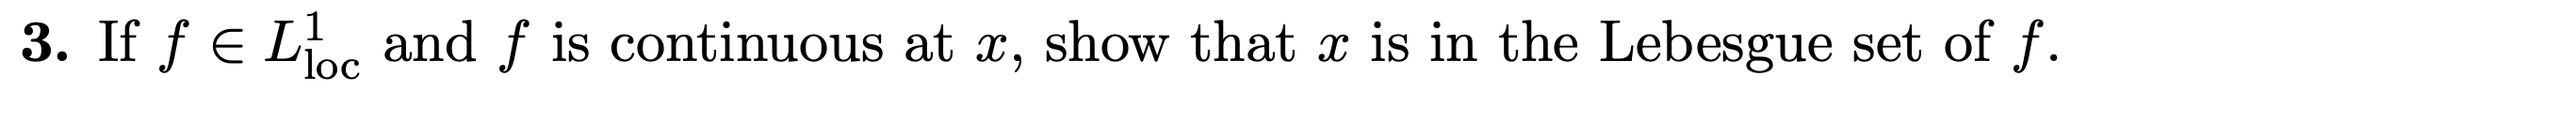
\includegraphics[width=400pt]{img/analysis--berkeley-202a-hw12-80ad.png}
\end{mdframed}

\begin{proof}
  Define $d_x(u) := f(u) - f(x)$. Using the notation $(A_r f)(x)$ to denote the average value of $f$
  on $B(x, r)$, we have
  \begin{align*}
    (A_r |d_x|)(x) = \frac{1}{m(B(x, r))} \int_{B(x, r)} |f(u) - f(x)| \du.
  \end{align*}
  We must show that $\lim_{r \to 0} (A_r |d_x|)(x) = 0$.

  Define $(S_r |d_x|)(x) := \origsup_u \big\{|f(u) - f(x)| ~:~ u \in B(x, r)\big\}$ and note
  that $(A_r |d_x|)(x) \leq (S_r|d_x|)(x)$ for all $r > 0$ (informally: the average cannot exceed the
  supremum).

  Therefore it suffices to show that $\lim_{r \to 0} (S_r |d_x|)(x) = 0$.

  Let $\eps > 0$. Since $f$ is continuous at $x$ we have that there exists $R > 0$ such
  that $f(B(x, R)) \subseteq B(f(x), \eps)$. Therefore for all $r \leq R$ we have $(S_r |d_x|)(x) < \eps$.
  Therefore $\lim_{r \to 0} (S_r |d_x|)(x) < \eps$.

  Since $\eps$ is arbitrary we have $\lim_{r \to 0} (S_r |d_x|)(x) = 0$ as required.
\end{proof}

[Did I use $f \in L^1_{\text{loc}}$?]


\newpage
\begin{mdframed}
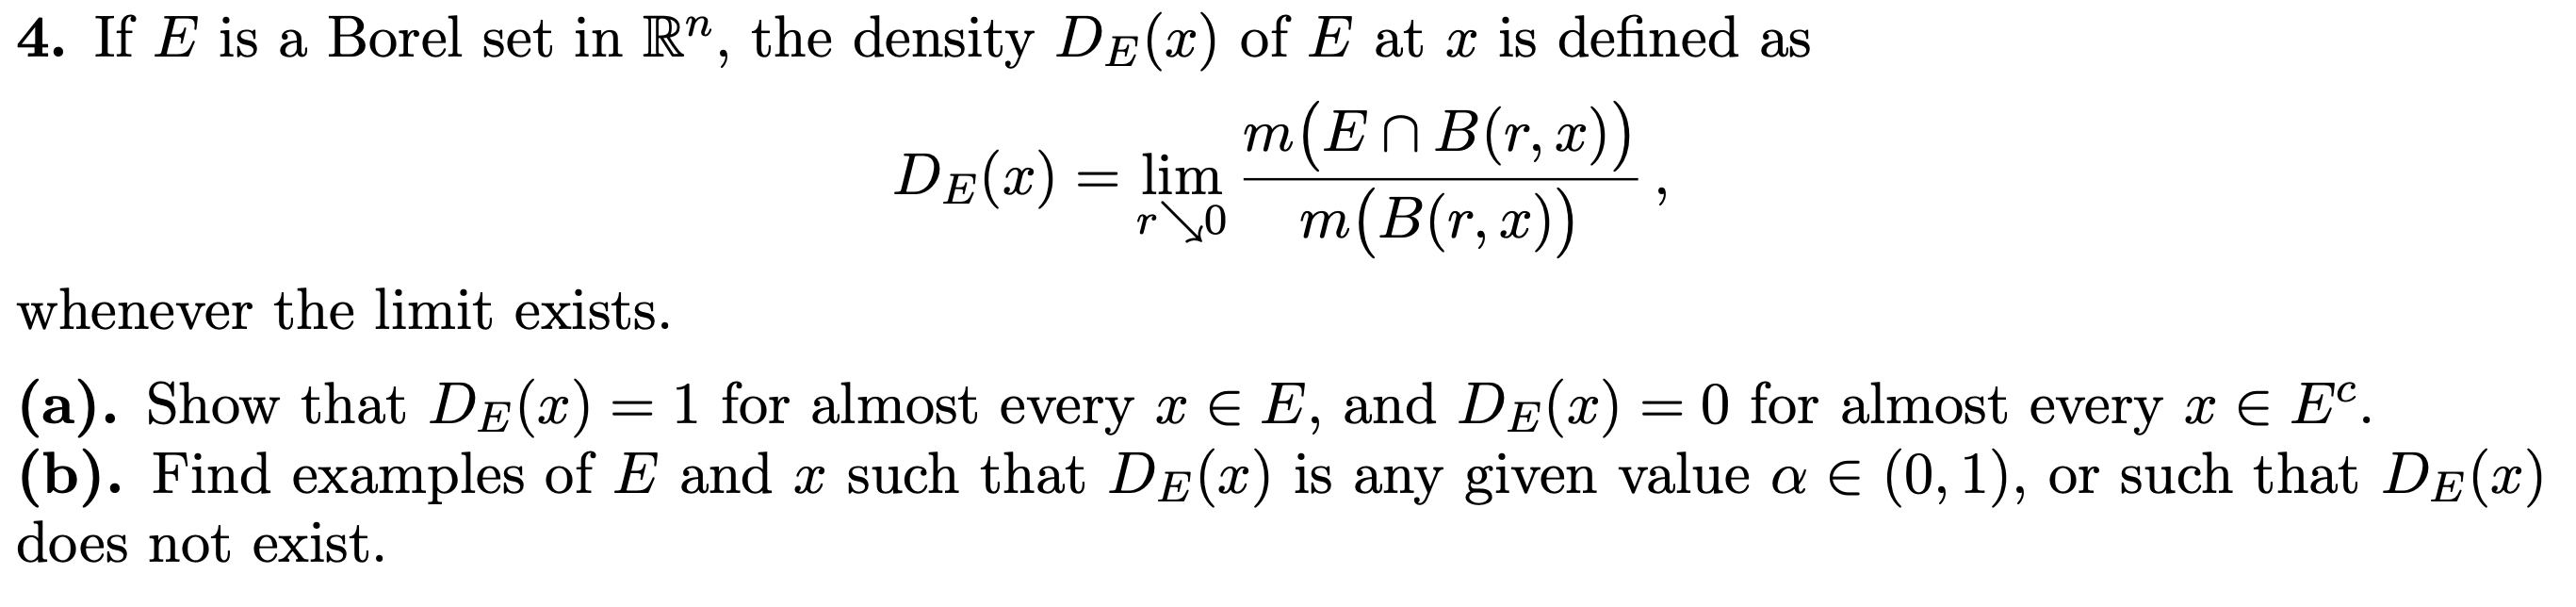
\includegraphics[width=400pt]{img/analysis--berkeley-202a-hw12-3d8f.png}
\end{mdframed}

\begin{enumerate}[label=(\alph*)]
\item
  \begin{claim*}
    $D_E(x) = 1$ for almost all $x \in E$.
  \end{claim*}

  \begin{proof}
    Since $E$ is a Borel set, almost every point of $E$ is in the interior of an open set. Let $x \in O^o$ be
    such a point, in the interior of an open set $O \subseteq E$. Then there exists $R > 0$ such
    that $B(x, r) \subset O$ for all $r < R$. Therefore
    \begin{align*}
      D_E(x)
      &:= \lim_{r \searrow 0} \frac{m(E \cap B(x, r))}{m(B(x, r))} \\
      &= \lim_{r \searrow 0} \frac{m(B(x, r))}{m(B(x, r))} \\
      &= 1.
    \end{align*}
  \end{proof}

  \begin{claim*}
    $D_E(x) = 0$ for almost all $x \in E^c$.
  \end{claim*}

  \begin{proof}
    Since $E$ is a Borel set, almost every point of $E^c$ is in the interior of a closed set. Similar proof to
    that just given.
  \end{proof}

\item
  \begin{claim*}
    Let $\alpha \in (0, 1)$. A set $E$ and a point $x$ exist such that $D_E(x) = \alpha$.
  \end{claim*}

  \begin{proof}
    This example only works for dimension $n > 1$. Basically, we make pie slices.

    In $\R^2$, let $E = \{(r, \theta) ~:~ \theta < 2\pi\alpha\}$, and let $x = (0, 0)$. Then
    \begin{align*}
      D_E(x)
      &= \lim_{r \to 0} \frac{m(E \cap B(x, r))}{m(B(x, r))} \\
      &= \lim_{r \to 0} \frac{\alpha\pi r^2}{\pi r^2} \\
      &= \alpha.
    \end{align*}
    For $n > 1$ in general, we can do the same thing: we have an $(n-1)$-dimensional hypersphere, and we select
    a hyperspherical sector whose volume relative to the volume of the hypersphere is $\alpha$. We define $E$
    to be the set of points in that hyperspherical sector.
  \end{proof}

  \begin{remark*}
    One could make a probabilistic construction in which each point $x$ is included in $E$ with
    probability equal to $|x|$:
    \begin{align*}
      E := \{x \in \R^n ~:~ |x| < \text{Bern}(|x|), |x| \leq 1\}.
    \end{align*}
    For such an $E$ it would (I claim) be true almost surely that $D_E(x) = \alpha$ for all $x$ such
    that $|x| = \alpha$, but such an $E$ would not (in general?) be a Borel set.

    Recall that it is not possible to construct a measurable set with measure $\alpha \in (0, 1)$ everywhere.
    The proof is by contradiction: we can cover our set with an open set to arbitrarily high efficiency; but
    this open set can be written as the countable union of intervals, and so this arbitrarily high density can
    be written as a weighted average of densities in intervals, and yet the density in each interval
    is $\alpha$.
  \end{remark*}



  \begin{claim*}
     A set $E$ exists and a point $x$ exist such that $D_E(x)$ does not exist.
  \end{claim*}

  \begin{proof}
    Let $E = \{u \in \R ~:~ \sin(|u|^{-1}) > 0\}$ and let $x = 0$.
  \end{proof}
\end{enumerate}






\newpage
\begin{mdframed}
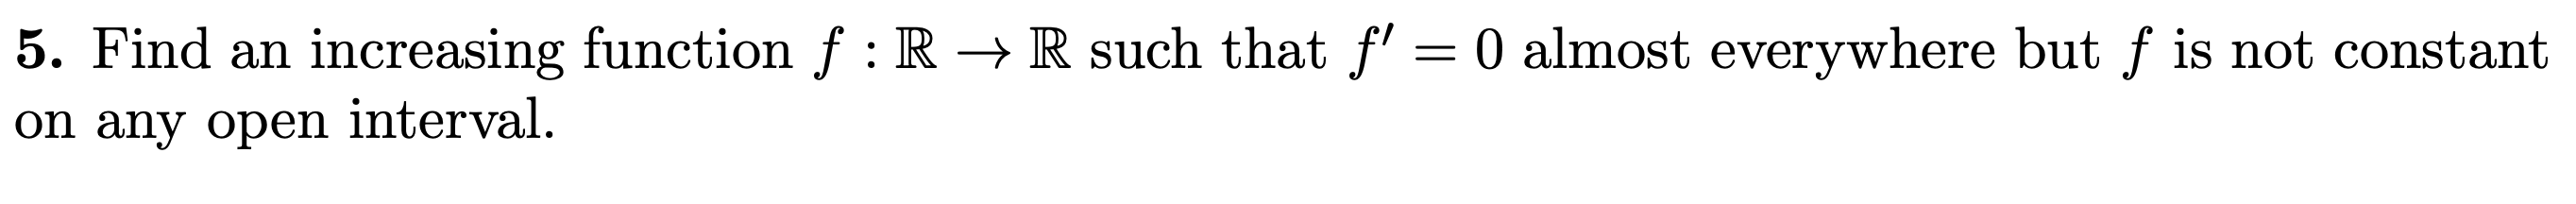
\includegraphics[width=400pt]{img/analysis--berkeley-202a-hw12-010d.png}
\end{mdframed}

\begin{proof}
  Some modification of the Cantor-Lebesgue function?
\end{proof}